% !TeX program = xelatex
% Build from this directory with: xelatex devs_tutorial.tex
\documentclass[11pt,a4paper]{article}
\usepackage[margin=22mm]{geometry}
\usepackage{fontspec}
\usepackage{xcolor,amsmath,fancyvrb,graphicx}
\usepackage[hidelinks]{hyperref}
\definecolor{ink}{HTML}{152B42}
\definecolor{accent}{HTML}{185C67}
\setlength{\parindent}{0pt}
\setlength{\parskip}{5pt}
\raggedbottom
\newcommand{\api}[1]{\texttt{#1}}
\newcommand{\figurelabel}[1]{\refstepcounter{figure}{\small\textbf{Figure \thefigure.} #1}}
\newcommand{\partmark}[1]{\par\noindent{\large\color{accent}\bfseries #1}\par\smallskip}
\newcommand{\chaptermark}[1]{\par\noindent{\LARGE\color{ink}\bfseries #1}\par\smallskip}
\newcommand{\topic}[1]{\par\medskip{\large\color{accent}\bfseries #1}\par}
\DefineVerbatimEnvironment{Code}{Verbatim}{fontsize=\footnotesize,frame=leftline,framesep=6pt}
\hypersetup{pdftitle={DEVS in SOCS},pdfsubject={A tutorial on the SOCS simulation models}}
\begin{document}

{\fontsize{34}{39}\selectfont\color{ink}\bfseries DEVS in SOCS}\par
{\large A hands-on introduction to atomic, coupled, and continuous models}\par
\vspace{3mm}{\color{accent}\hrule}\vspace{4mm}

Run the commands from the SOCS repository root in a Python 3.13 environment.
If the package has not been installed in that environment, run
\api{python -m pip install -e .} first. Live windows use Tkinter.
Live phase diagrams also use the Graphviz \api{dot} executable.
Make it available on \api{PATH} or install it in the standard Windows
Graphviz location recognized by SOCS.

\partmark{Part 1 \enspace Discrete Event System}
\chaptermark{Chapter 1 \enspace Timed Event System}
\begin{center}
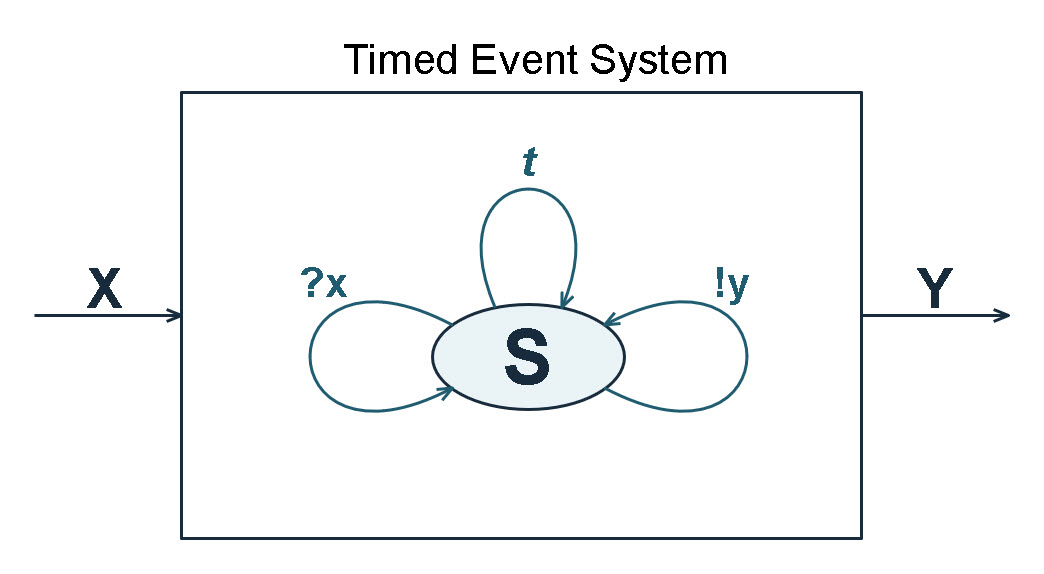
\includegraphics[width=.94\linewidth,height=10cm,keepaspectratio]{images/TimedEventSystem.jpg}\par
\figurelabel{Timed Event System}
\end{center}
\begin{equation}
TES = (X, Y, S, s_0, \Delta_t, \Delta_x, \Delta_y)
\label{eq:tes}
\end{equation}
where
\begin{itemize}
  \item $X$ is the set of input events.
  \item $Y$ is the set of output events.
  \item $S$ is the set of states.
  \item $s_0 \in S$ is the initial state.
  \item $\Delta_t: S \times T \rightarrow S$ is the continuous transition function, here  $T=[0,\infty)$ is a set of non-negative real numbers representing $times$. 
  \item $\Delta_x: S \times T \times X \rightarrow S$ is the external transition function defining how the system changes its state when it receives an input event at a certain time.
  \item $\Delta_y: S \times T \rightarrow S\times Y$ is the internal transition function defining how the system changes its state and generates an output event at a certain time. 
\end{itemize}
\newpage
\chaptermark{Chapter 2 \enspace DEVS}
\begin{center}
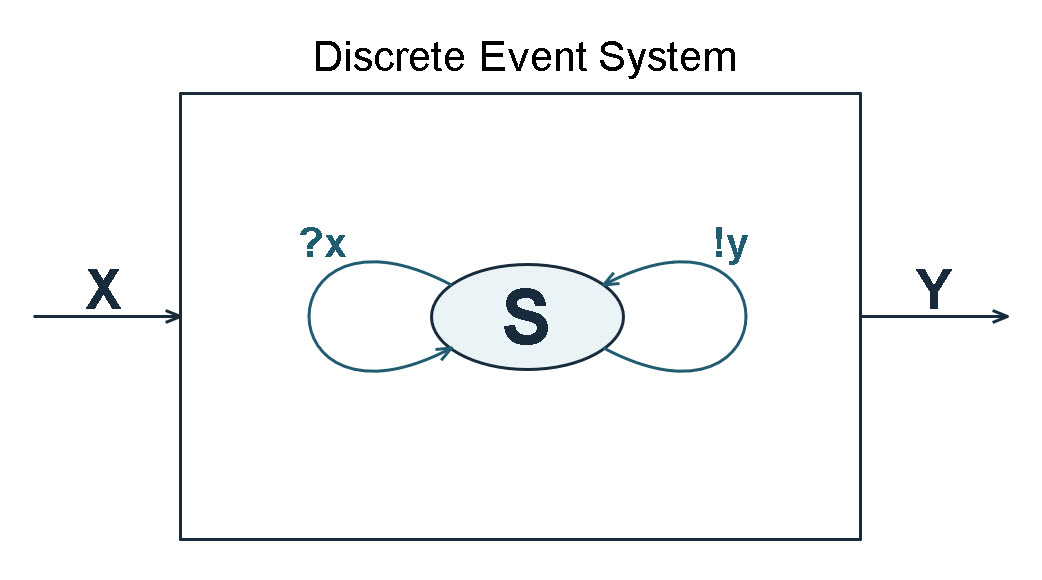
\includegraphics[width=.94\linewidth,height=10cm,keepaspectratio]{images/DEVS.jpg}\par
\figurelabel{DEVS}
\end{center}

\begin{equation}
DEVS=(X, Y, S, s_0, \delta_x, \delta_y, \tau)
\label{eq:devs}
\end{equation}
\begin{itemize}
	\item $X$ is the set of input events.
	\item $Y$ is the set of output events.
	\item $S$ is the set of states.
	\item $s_0 \in S$ is the initial state. 
	\item $\delta_x: S \times X \rightarrow S$ is the external transition function defining how the system changes its state when it receives an input event at a certain time.
	\item $\delta_y: S \rightarrow S\times Y$ is the internal transition function defining how the system changes its state and generates an output event at a certain time. 
\end{itemize}
\newpage
\chaptermark{2.1 \enspace DEVS}

An \emph{atomic} DEVS model defines its own state and transitions. A
\emph{coupled} model connects the ports of atomic or other coupled
models. SOCS passes an event as \api{PortValue(port, value)}, where
the port name is a string and the value may be omitted.

\topic{2.1.1 \enspace DEVSCounter}
\begin{Code}
python -m examples.DEVS_Simple.DEVSCounter --count 3
\end{Code}
Read the \api{Counter} class in \api{DEVSCounter.py}. \api{set\_initial\_state()}
initializes the model. \api{tau()} gives the time until its next internal
event. At each scheduled event, \api{delta\_y()} returns the current sum
on \api{!c}, adds the next integer, and increments the counter. After
the requested count, the model enters Done, with $\tau=\infty$.

\begin{Code}
def set_initial_state(self):
        """Initialize the counter state."""
        self.phase, self.count, self.sum = "C", 1, 0

def tau(self):
        """Return the time until the next internal event."""
        if self.phase == "C":
            return 5
        return float("inf")

def delta_x(self, event: PortValue) -> bool:
    """Ignore external events because this counter has no inputs."""
    return False

def delta_y(self) -> PortValue:
        """Emit the current sum, then update the counter state."""
        output = PortValue(self.OP["!c"], self.sum)
        if self.phase == "C":
            self.sum += self.count
            self.count += 1
            if self.count > self.count_no:
                self.phase = "D"
        return output
\end{Code}
Every concrete \api{DEVS} model implements \api{set\_initial\_state()},
\api{tau()}, \api{delta\_x()}, and \api{delta\_y()}. This counter's
\api{delta\_x()} ignores the input and returns \api{False}.

\begin{Code}
t=5  phase=Count count=1 sum=1 !c=0
t=10 phase=Count count=2 sum=3 !c=1
t=15 phase=Done  count=3 sum=6 !c=3
\end{Code}
The \api{sum} column is the updated state. The \api{!c} value is the
sum emitted just before that update. Add \api{--live} to see the phase
and remaining time while the same simulation runs.

\newpage
\chaptermark{2.1 \enspace DEVS, continued}
\topic{2.1.2 \enspace DEVSToaster}
\begin{Code}
python -m examples.DEVS_Simple.DEVSToaster --live
\end{Code}
Press \textbf{Push} to inject \api{?push}. The default toasting time
is 10 seconds. Use \api{--toasting-time 5} for a five-second run. In
console mode, Enter starts a cycle and \api{q} exits.

When the toaster is idle, \api{delta\_x()} changes the phase to
Toasting and returns \api{True}. SOCS schedules the next internal
event at the input time plus the new phase's \api{tau()}. A second
push during Toasting returns \api{False} and preserves the original
deadline. When that deadline arrives, \api{delta\_y()} emits
\api{!pop} and returns the toaster to Idle.

\begin{Code}
def set_initial_state(self):
        """Reset the toaster to its initial idle phase."""
        self.phase = "Idle"

def tau(self):
        """Return the time until the next internal event."""
        if self.phase == "Toasting":
            return self.tt
        return inf

def delta_x(self, x):
        """Handle a push event and reschedule if toasting starts."""
        if isinstance(x, PortValue) and x.port == "?push" and self.phase == "Idle":
            self.phase = "Toasting"
            return True
        return False

def delta_y(self):
        """Emit the pop event and return to the idle phase."""
        if self.phase == "Toasting":
            self.phase = "Idle"
            return PortValue("!pop")
        return None
\end{Code}
Console result after pressing Enter with the default ten-second setting.
\begin{Code}
t=0 Idle> t=0 Toasting
t=10 Idle !pop
\end{Code}

\newpage
\chaptermark{2.1 \enspace DEVS, continued}
\topic{2.1.3 \enspace DEVSPingPong}
\begin{Code}
python -m examples.DEVS_Simple.DEVSPingPong
\end{Code}
Choose \api{s} at the example menu to enter the simulator.
Player A starts Sending and takes 0.1 time units to send.
Player B starts Waiting and takes 0.2 time units once it receives
the ball. Each player emits \api{!s} on a send and receives
\api{?r} from the other player.

\begin{Code}
def set_initial_state(self):
        """Initialize the player's phase."""
        self.phase = self.initial_phase

def tau(self):
        """Return the time until the next internal event."""
        if self.phase == "S":
            return self.send_time
        return float("inf")

def delta_x(self, x):
        """Handle a received ball and request rescheduling when needed."""
        if x.port == "?r" and self.phase == "W":
            self.phase = "S"
            return True
        return False

def delta_y(self):
        """Send the ball and transition to the waiting phase."""
        if self.phase == "S":
            self.phase = "W"
            return PortValue(self.OP["!s"])
        return None
\end{Code}
\begin{Code}
model.addOutputPorts("!ping", "!pong")
model.addCouples(
    ((player_a, "!s"), (player_b, "?r")),
    ((player_b, "!s"), (player_a, "?r")),
    ((player_a, "!s"), (model, "!ping")),
    ((player_b, "!s"), (model, "!pong")),
)
\end{Code}
An endpoint is a pair of a model and a port name. A's output travels
both to B's input and to the coupled boundary's \api{!ping} port.
B's output travels both to A's input and to \api{!pong}. The boundary
outputs alternate at $t=0.1,\ 0.3,\ 0.4,\ 0.6,\ldots$.

\begin{Code}
t=0.1  !ping
t=0.3  !pong
t=0.4  !ping
t=0.6  !pong
\end{Code}
\topic{What the live view does}
The view passes user input to the engine, runs simulation steps, and
draws the resulting model state. The model class defines the behavior.
For the tutorial, the important connection is input $\to$ engine
$\to$ updated model $\to$ view.

\newpage
\chaptermark{2.2 \enspace DEVSph}
\begin{equation}
DEVS_{ph}=(X, Y, S_{p}, \delta_{0,p}, \delta_{0,p}, \delta_{0,p})
\label{eq:devsph}
\end{equation}

DEVSph and cDEVSph examples open a live window by default. \api{--live} is explicit; use \api{--console} for a text run.


\api{DEVSph} lets you declare a phase graph. Each node holds a phase
name and its \api{tau}. Each directed edge describes an internal or
external transition. SOCS uses the declared \api{AGraph} to select
the transitions, and the live view uses it to draw the diagram.

\topic{2.2.1 \enspace DEVSphToaster}
\begin{Code}
python -m examples.DEVS_Simple.DEVSphToaster --live
\end{Code}
In the external-event panel, select \api{Toaster} and \api{?push},
leave \textbf{Value (JSON)} empty, and click \textbf{Apply}.
The empty value becomes Python \api{None}. The example uses this
declaration.

\begin{Code}
self.add_phase("Idle", tau=inf, initial=True)
self.add_phase("Toasting", tau=toasting_time)
self.add_external_transition(
    "Idle", "Toasting", input_port="?push", reschedule=True,
)
self.add_internal_transition("Toasting", "Idle", output="!pop")
\end{Code}
Only Idle has a \api{?push} edge. A push while Toasting leaves the
state and schedule as they were, so it has no edge in the diagram.
In \textbf{DEVS Only} mode, Apply delivers the external event and
\textbf{Step} executes the next scheduled internal event. In
\textbf{Animation} mode, the display updates at intervals of 0.1
simulation seconds during toasting.

\topic{Reading the diagram}
The entry arrow marks the initial phase. A fill marks the current
phase and its remaining time is $t_{\mathrm{next}}-t_{\mathrm{now}}$.
An infinite-\(\tau\) phase has a dashed outline. Internal transitions
and external transitions with \api{reschedule=True} use solid lines.
External transitions with \api{reschedule=False} use dashed lines.
A dashed self-loop can describe an update to model data while the
phase and scheduled time stay the same.

\begin{center}
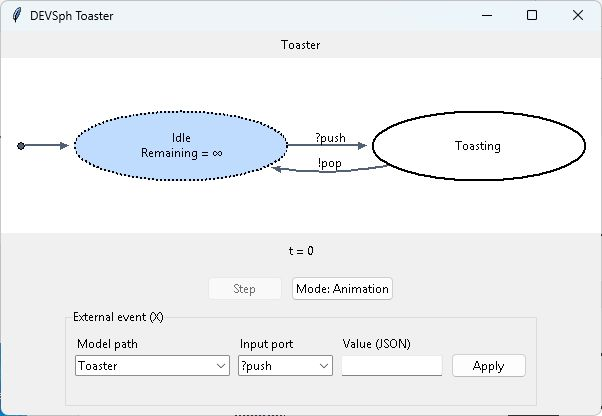
\includegraphics[width=.92\linewidth,height=6.7cm,keepaspectratio]{images/toaster.jpg}\par
\figurelabel{Toaster input panel. Leave Value blank and click Apply.}
\end{center}

\newpage
\chaptermark{2.2 \enspace DEVSph, continued}
\topic{2.2.2 \enspace DEVSphPingPong}
\begin{Code}
python -m examples.DEVS_Simple.DEVSphPingPong --live
\end{Code}
The two diagrams are titled \api{PingPong.A} and \api{PingPong.B}.
Select \textbf{Show Coupling} to read all four connections.
The Animation interval is 0.01 simulation time units. In
\textbf{DEVS Only} mode, Step advances to the next send.
With \api{--console}, the command accepts \api{--steps 4} to print four sends.

\begin{Code}
self.addInputPorts("?r")
self.addOutputPorts("!s")
self.add_phase("Sending", tau=send_time, initial=starts)
self.add_phase("Waiting", tau=inf, initial=not starts)
self.add_external_transition(
    "Waiting", "Sending", input_port="?r", reschedule=True,
)
self.add_internal_transition("Sending", "Waiting", output="!s")
\end{Code}
To inject a ball receipt, select \api{PingPong.B} and \api{?r}, leave Value blank, and press Apply. Only Waiting has a receive transition. Leave the input panel untouched when comparing the regular rally times.
\begin{center}
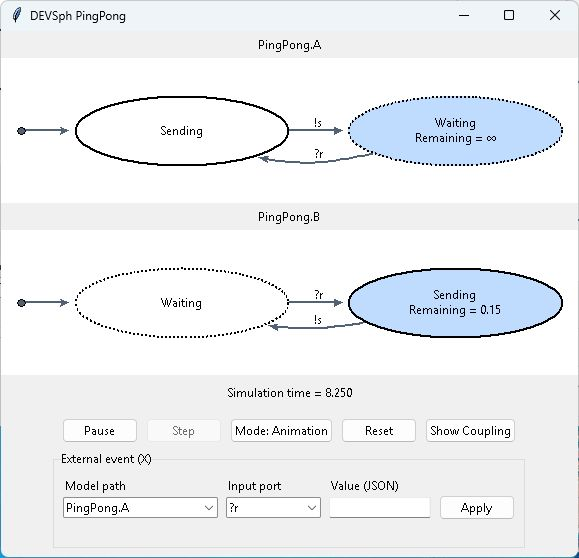
\includegraphics[width=.92\linewidth,height=8.3cm,keepaspectratio]{images/pingpong.jpg}\par
\figurelabel{Both players, execution mode, coupling control, and external-event input.}
\end{center}

\newpage
\chaptermark{2.2 \enspace DEVSph, continued}
\topic{2.2.3 \enspace DEVSphCounterBasic}
\begin{Code}
python -m examples.DEVS_Simple.DEVSphCounterBasic --live --count 3
\end{Code}
One graph node represents each complete state of this counter.
The label lists the phase name, completed count, and running sum.
\begin{equation}
 \mathrm{Count}(0,0)\ \longrightarrow\
 \mathrm{Count}(1,1)\ \longrightarrow\
 \mathrm{Count}(2,3)\ \longrightarrow\
 \mathrm{Done}(3,6)
\label{eq:counter-states}
\end{equation}
Each Count node has a five-unit time advance and one outgoing
internal transition. The edge can carry a fixed output such as
\api{PortValue("!c", 0)}. The destination node already represents the
updated count and sum, so this example requires no guard or action.

Here are the first two nodes and the first edge, expanded from the construction loop.
\begin{Code}
self.addOutputPorts("!c")
self.add_phase("Count(0, 0)", tau=5, initial=True)
self.add_phase("Count(1, 1)", tau=5)
self.add_internal_transition(
    "Count(0, 0)", "Count(1, 1)", output=PortValue("!c", 0),
)
\end{Code}
\begin{center}
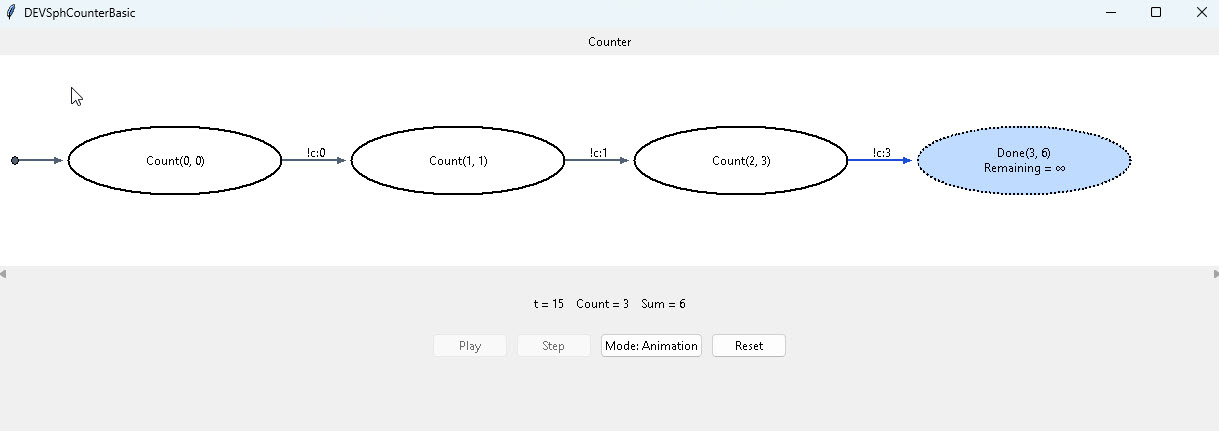
\includegraphics[width=.92\linewidth,height=7.5cm,keepaspectratio]{images/counter_basic.jpg}\par
\figurelabel{The view follows the active node. Use the horizontal scrollbar to see the earlier nodes.}
\end{center}

\newpage
\chaptermark{2.2 \enspace DEVSph, continued}
\topic{2.2.4 \enspace DEVSphCounter}
\begin{Code}
python -m examples.DEVS_Simple.DEVSphCounter --live --count 3
\end{Code}
The same counter can use two phase nodes and keep the count and sum
in \api{self.\_variable}. From Count there are two internal edges.

\begin{Code}
self.addOutputPorts("!c")
self.add_phase("Count", tau=5, initial=True)
self.add_phase("Done", tau=inf)
self.add_internal_transition(
    "Count", "Count", guard=self.has_more_ticks,
    action=self.increment, output=self.emit_sum,
)
self.add_internal_transition(
    "Count", "Done", guard=self.is_last_tick,
    action=self.increment, output=self.emit_sum,
)
\end{Code}
A \api{guard(model, event)} is a predicate that enables an edge.
An \api{action(model, event)} updates the model for the selected edge.
An internal transition passes \api{None} as its event. \api{DEVSph}
selects one enabled edge, evaluates its output on the source state,
runs its action, and sets the destination phase. The diagram labels
each edge with its guard and action names when present.

\begin{Code}
@staticmethod
def has_more_ticks(model, event):
    return model._variable.count + 1 < model.count_no

@staticmethod
def is_last_tick(model, event):
    return not model.has_more_ticks(model, event)

@staticmethod
def increment(model, event):
    model._variable.count += 1
    model._variable.sum += model._variable.count
\end{Code}

On the third tick, \api{is\_last\_tick} selects Count $\to$ Done.
\api{emit\_sum} sends 3, then \api{increment} sets the count to 3 and
the sum to 6. Try both counter examples in DEVS Only mode and compare
the output sequence and event times with Section 2.1.1.

Neither counter has an external input port. Use Play/Pause, Step, Mode, and Reset to control execution.
\begin{center}
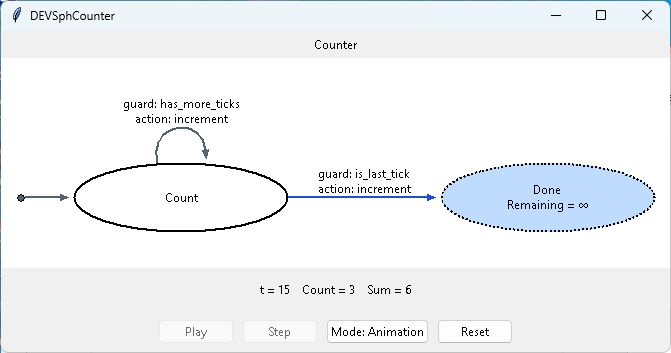
\includegraphics[width=.92\linewidth,height=5.1cm,keepaspectratio]{images/counter.jpg}\par
\figurelabel{The two Count edges are labeled with their guard and action names.}
\end{center}

\newpage
\partmark{Part 2 \enspace Continuous and Discrete Event System}
\chaptermark{Chapter 3 \enspace Continuous and Discrete Event System}
\begin{center}
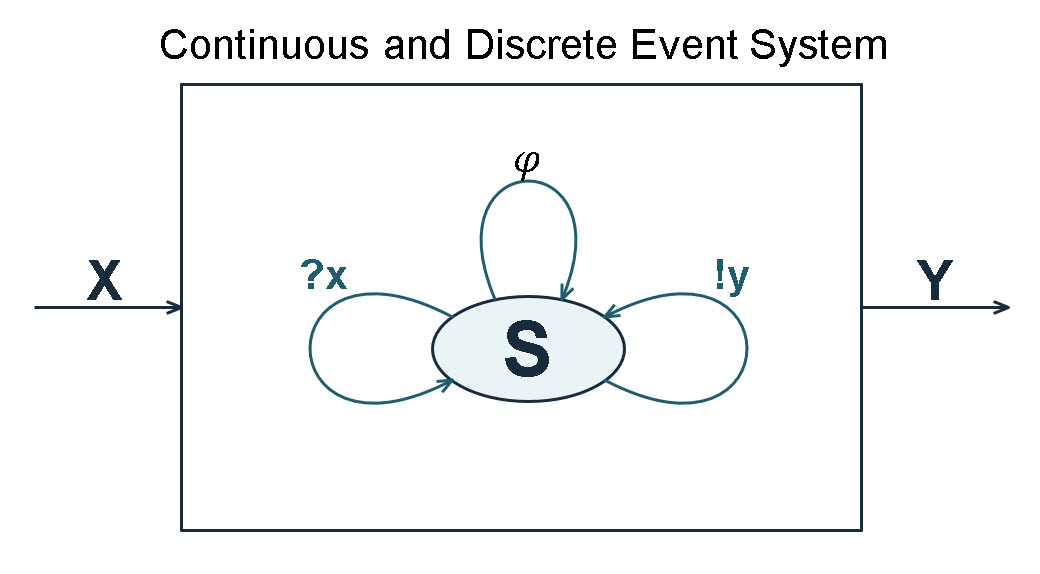
\includegraphics[width=.94\linewidth,height=10cm,keepaspectratio]{images/CDEVS.jpg}\par
\figurelabel{Continuous and Discrete Event System}
\end{center}

\newpage
\chaptermark{cDEVS and cDEVSph}

\api{cDEVS} adds the model hook \api{delta\_cont(elapsed)}.
\api{cDEVSph} combines that hook with a declared phase graph.
When the engine reaches a new simulation time, it calls
\api{Delta\_null(t)} before processing the events due there. The
continuous model advances over the elapsed interval with the
current phase's dynamics. At a shared event time, the engine performs
that time update once before handling the due events in order.
A finite simulation bound also advances the model to the bound.

\topic{cDEVSphElevator}
\begin{Code}
python -m examples.DEVS_Simple.cDEVSphElevator --live
\end{Code}
The car starts at floor 1. Apply \api{Elevator}, \api{?floor},
and JSON value \api{2} to send it upstairs. At arrival, send
\api{1} to return. Enter the floor number without quotation marks.
With \api{--console}, the example runs a round trip and prints the phase boundaries.

\begin{equation}
 \mathrm{Idle}\ \longrightarrow\ \mathrm{Accelerating}\
 \longrightarrow\ \mathrm{Cruising}\ \longrightarrow\
 \mathrm{Braking}\ \longrightarrow\ \mathrm{Idle}
\label{eq:elevator-phases}
\end{equation}
The floors are 3 m apart. A trip accelerates for 0.5 s, cruises at
1.5 m/s for 1.5 s, and brakes for 0.5 s. The phase edges switch
dynamics at $t=0.5,\ 2.0,\ 2.5$ s for the first trip.
The final edge emits \api{!arrived} with the target floor number.

\begin{Code}
self.add_phase("Idle", tau=inf, initial=True)
self.add_phase("Accelerating", tau=self.RAMP_TIME)
self.add_phase("Cruising", tau=self.FLOOR_HEIGHT / self.TOP_SPEED
               - self.RAMP_TIME)
self.add_phase("Braking", tau=self.RAMP_TIME)
self.add_external_transition(
    "Idle", "Accelerating", input_port="?floor", reschedule=True,
    match=lambda floor: type(floor) is int and floor in (1, 2),
    guard=self.is_different_floor, action=self.set_target,
)
self.add_internal_transition("Accelerating", "Cruising")
self.add_internal_transition("Cruising", "Braking")
self.add_internal_transition(
    "Braking", "Idle", action=self.finish_trip,
    output=lambda model: PortValue("!arrived", model._variable.target),
)
\end{Code}

After the input matches a valid floor number, the guard checks that it differs from the current floor. The first action stores the target. The arrival action updates the floor, position, and velocity.
\begin{Code}
@staticmethod
def is_different_floor(model, event):
    return event.value != model._variable.floor

@staticmethod
def set_target(model, event):
    model._variable.target = event.value

@staticmethod
def finish_trip(model, event):
    target = model._variable.target
    model._variable.update(
        floor=target, position=(target - 1) * model.FLOOR_HEIGHT,
        velocity=0.0,
    )
\end{Code}

\newpage
\chaptermark{cDEVS and cDEVSph, continued}
\topic{The motion inside a phase}
\api{tNow} is the simulation time being evaluated. \api{tLast} is the
model's scheduling reference time. For this elevator, it is the start
time of the current phase. If acceleration begins at \(t=0\), then at
the animation tick at \(t=0.10\), \api{tNow} is 0.10 and \api{tLast}
is still 0. The elapsed time is \(\Delta t=\api{tNow}-\api{tLast}=0.10\) s.

With constant acceleration \(a\), \api{delta\_cont()} evaluates motion
from the phase's starting position \(x_L\) and velocity \(v_L\).
\begin{equation}
 x(t) = x_L+v_L\Delta t+\tfrac12 a(\Delta t)^2,\qquad
 v(t) = v_L+a\Delta t .
\label{eq:elevator-motion}
\end{equation}
The signs of velocity and acceleration account for travel direction.
The model finishes each trip at the target floor with zero velocity.

\begin{Code}
def delta_cont(self, elapsed):
    """Evaluate motion at elapsed seconds after the current phase began."""
    if self.phase == "Idle":
        return
    state = self._variable
    direction = state.target - state.floor
    start = (state.floor - 1) * self.FLOOR_HEIGHT
    ramp_distance = self.TOP_SPEED * self.RAMP_TIME / 2
    acceleration = self.TOP_SPEED / self.RAMP_TIME
    if self.phase == "Accelerating":
        distance = acceleration * elapsed**2 / 2
        speed = acceleration * elapsed
    elif self.phase == "Cruising":
        distance = ramp_distance + self.TOP_SPEED * elapsed
        speed = self.TOP_SPEED
    else:
        distance = (self.FLOOR_HEIGHT - ramp_distance
                    + self.TOP_SPEED * elapsed)
        distance -= acceleration * elapsed**2 / 2
        speed = self.TOP_SPEED - acceleration * elapsed
    state.position = start + direction * distance
    state.velocity = direction * speed
\end{Code}
Each animation tick evaluates motion from the same origin. Scheduled
discrete transitions switch phases and emit \api{!arrived}.
\topic{Two views of one simulation}
The phase diagram shows the current phase and remaining time.
The shaft view maps the same model's position from meters to pixels.
The drawing code is in \api{\_elevator\_view.py}.

\begin{center}
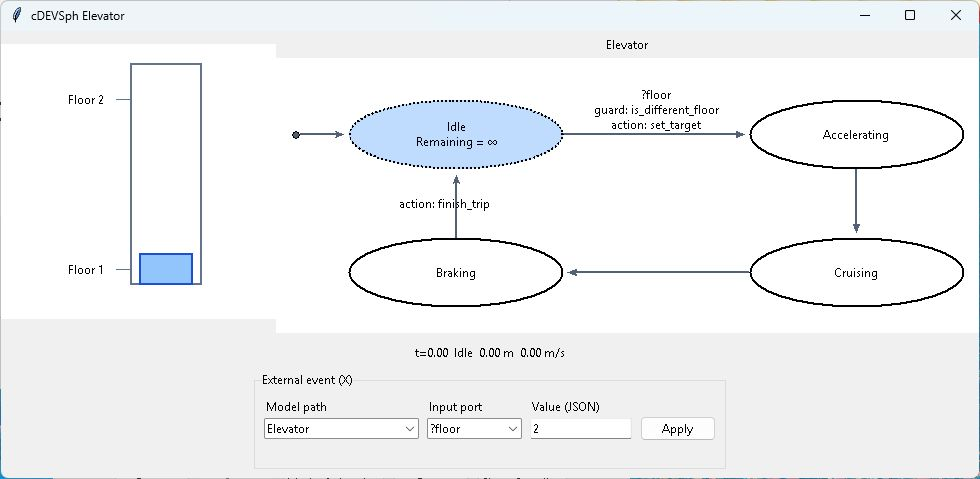
\includegraphics[width=.92\linewidth,height=5.4cm,keepaspectratio]{images/elevator.jpg}\par
\figurelabel{The elevator at floor 1. Apply the prefilled value 2 to start accelerating.}
\end{center}

\end{document}
